\documentclass{standalone}

\usepackage{tikz}

\begin{document}
  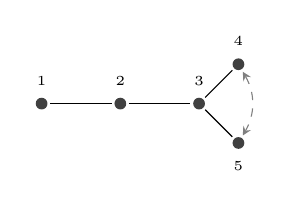
\begin{tikzpicture}
    \tikzstyle{v1} = [color=darkgray, circle, outer sep=1pt, fill, inner sep=1.5pt]
    \tikzstyle{v2} = [color=darkgray, circle, outer sep=1pt, fill, inner sep=3.0pt]

    % See fig-well-rooted-E6.tex
    \tikzstyle{a} = [color=gray, dashed, <->, >={stealth}] \tikzset{font=\tiny}

    \node[v1, label={1}] (1) at (0,0) {};
    \node[v1, label={2}] (2) at (1,0) {};
    \node[v1, label={3}] (3) at (2,0) {};
    \node[v1, label={4}] (4) at (2.5, 0.5) {};
    \node[v1, label=270:{5}] (5) at (2.5,-0.5) {};
    \draw (1) -- (2);
    \draw (2) -- (3);
    \draw (3) -- (4);
    \draw (3) -- (5);
    \draw[a] (4) to[bend left] (5);
  \end{tikzpicture}
\end{document}
